% ============================================================================
%  HARDWARE PORTFOLIO -- hardware projects only
%  Siblings, under portfolio/:
%    ../software/   software only
%    ../general/    both
%    ../baykar/     hardware-led, written for a Baykar application
%  Images are shared, one level up in ../img/
%
%  Build from inside this directory:
%      pdflatex "Mohammed Aljomaily.tex"
% ============================================================================

\documentclass[11pt,a4paper]{article}

\usepackage[T1]{fontenc}
\usepackage{lmodern}
\usepackage[margin=1.9cm]{geometry}
\usepackage{enumitem}
\usepackage{graphicx}
\usepackage[hidelinks]{hyperref}

% Float placement tuning: prefer figures on pages that also carry text, and
% only build a dedicated figure page when it would be almost completely full.
\renewcommand{\topfraction}{0.92}
\renewcommand{\bottomfraction}{0.92}
\renewcommand{\textfraction}{0.06}
\renewcommand{\floatpagefraction}{0.9}

\setlength{\parindent}{2pt}
\setlength{\parskip}{5pt}
\pagestyle{empty}
\hyphenpenalty=1200
\exhyphenpenalty=1200
\emergencystretch=1.5em

\newcommand{\entry}[2]{%
  \vspace{6pt}%
  {\Large\bfseries #1}\hfill{\itshape\small #2}\par
  \vspace{3pt}\hrule\vspace{4pt}%
}

\begin{document}

\begin{center}
    {\LARGE \textbf{Mohammed Aljomaily}}\\[3pt]
    {\large Hardware Portfolio}\\[6pt]
    {\small Computer Engineering Student \textbar{} Embedded Systems, PCB Design \& RF}\\[3pt]
    {\small Beylikd\"uz\"u, Istanbul, Turkey \textbar{} +90 535 273 6199 \textbar{}
    \href{mailto:mohammedaljomaily06@gmail.com}{mohammedaljomaily06@gmail.com}}\\[2pt]
    {\small \href{https://v01d.dev}{v01d.dev} \textbar{} \href{https://github.com/V01Ddev}{github.com/V01Ddev}}
\end{center}

\entry{Preface}{}

I am a Computer Engineering student at Istanbul Ayd{\i}n University, and this is
a record of the hardware I have designed, built and flown.

I came into engineering through software, somewhat by accident. During a gap
year I took an internship at Applab in Doha, and it turned into fourteen months
of backend work for an AI video platform used by Al Jazeera. It was serious work
and I am proud of it, but it was never the part of engineering I went looking
for. The thing I actually did with my own time was different: designing circuit
boards, etching them at my kitchen table, soldering them, and flying what I had
built. This document is that work.

Over the past year I have designed and hand-etched my own PCBs at home, because
paying for fabrication and shipping to Turkey did not make sense for the size of
the boards I was making. I designed a two-layer ESP32 board carrying two
nRF24L01 transceivers on separate SPI buses, and discovered after the first
layout that two layers are close to impossible to produce by hand. I widened the
vias, reworked the routing, and made it again. The board works. I have built and
tuned a 5-inch FPV quadcopter and written the firmware for the radio link on my
fixed-wing designs. I published a KiCad footprint library for the SSD1306 OLED
because I needed one that worked in a current version of KiCad and could not
find it, and I use it in my own boards. I keep a written preflight checklist for
my aircraft, because I would rather catch a loose propeller on the bench than in
the air.

Almost everything here was made at a desk at home, including the circuit boards
themselves. Where a project is unfinished I have said so.

\entry{5-Inch FPV Quadcopter}{2026}

A complete 5-inch FPV aircraft, built from parts and configured from scratch:
\textbf{Mario 5} frame, \textbf{Mamba MK4 F722} flight controller, \textbf{F40 V2}
motors, and \textbf{DJI O4 Lite} video on \textbf{6S}. I configured Betaflight,
set up the \textbf{ExpressLRS 2.4\,GHz} control link between a RadioMaster Pocket
running EdgeTX and the receiver, and tuned the aircraft to fly the way I wanted
it to rather than the way it arrived.

I wrote the preflight checklist for this aircraft myself, as a ground-check
procedure I run before every session. It is not a formality: on a machine with
propellers, batteries and a radio link, the failures that hurt are the boring
ones.

Alongside the airframe I built out the rest of the workflow, including GyroFlow
stabilisation for footage from a GoPro HERO7 with ND filters, and a custom EdgeTX
sound pack and 3D-printed stick ends for the radio.

\begin{figure}[!htbp]
\centering
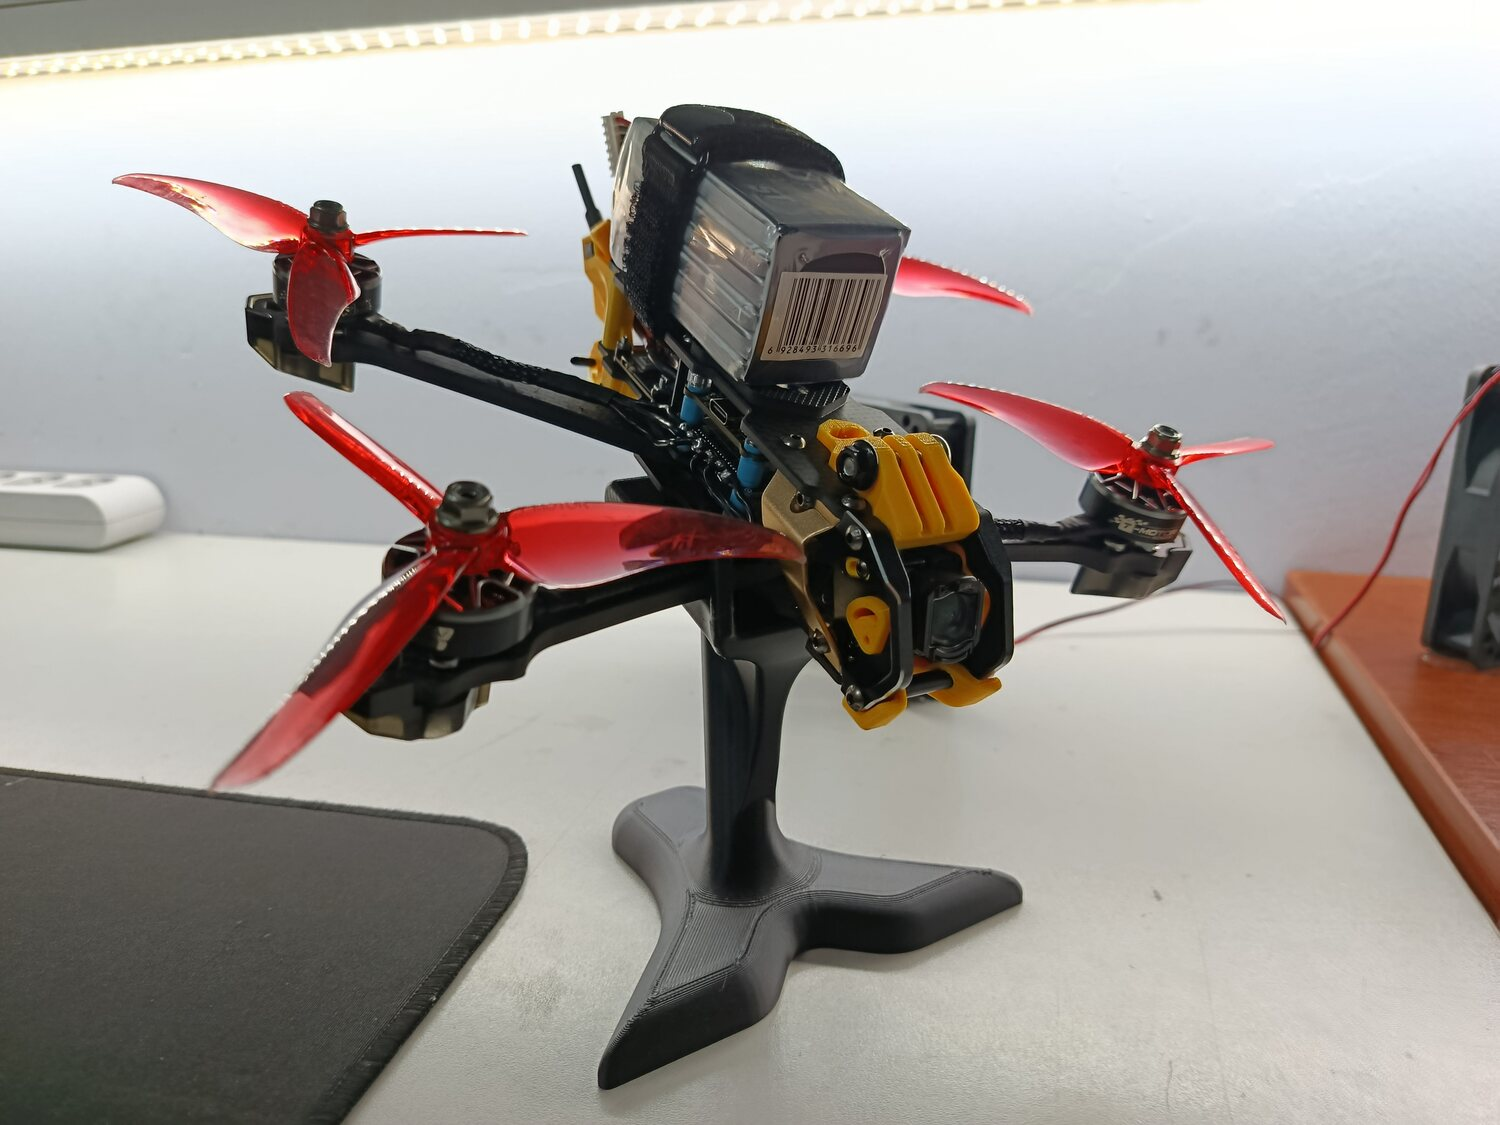
\includegraphics[width=0.38\textwidth]{../img/drone.jpg}
\caption{The finished 5-inch build.}
\end{figure}

\entry{Dual-Transceiver ESP32 Jammer Board}{2026}

A two-layer ESP32 jammer board I designed in \textbf{KiCad} for educational study
of 2.4\,GHz protocols, and then fabricated by hand at home: an \textbf{ESP32
DevKit V1} carrying \textbf{two nRF24L01+PA+LNA} transceivers, each on its own
SPI bus (HSPI and VSPI) so both radios operate independently, plus an SSD1306
OLED for status and an optional TP4056 charging circuit for a Li-Ion cell. The
finished board is 64.14 $\times$ 77.47\,mm.

I did not use a fabrication house. Shipping to Turkey plus the cost of a local
service made no sense for boards this size, so I generate the artwork, transfer
it, etch it, drill it and assemble it myself. That decision shaped the design:
the first layout was two layers and turned out to be close to impossible to
produce by hand, so I enlarged the vias, reworked the routing for the process,
cleared every DRC error, and made it a second time. The second board works.

The firmware is adapted from an existing open-source project rather than written
from scratch. I wanted my hardware to be fully compatible with it, so the
engineering work on my side was the board, the schematic capture, the custom
footprints and the fabrication.

\begin{figure}[!htbp]
\centering
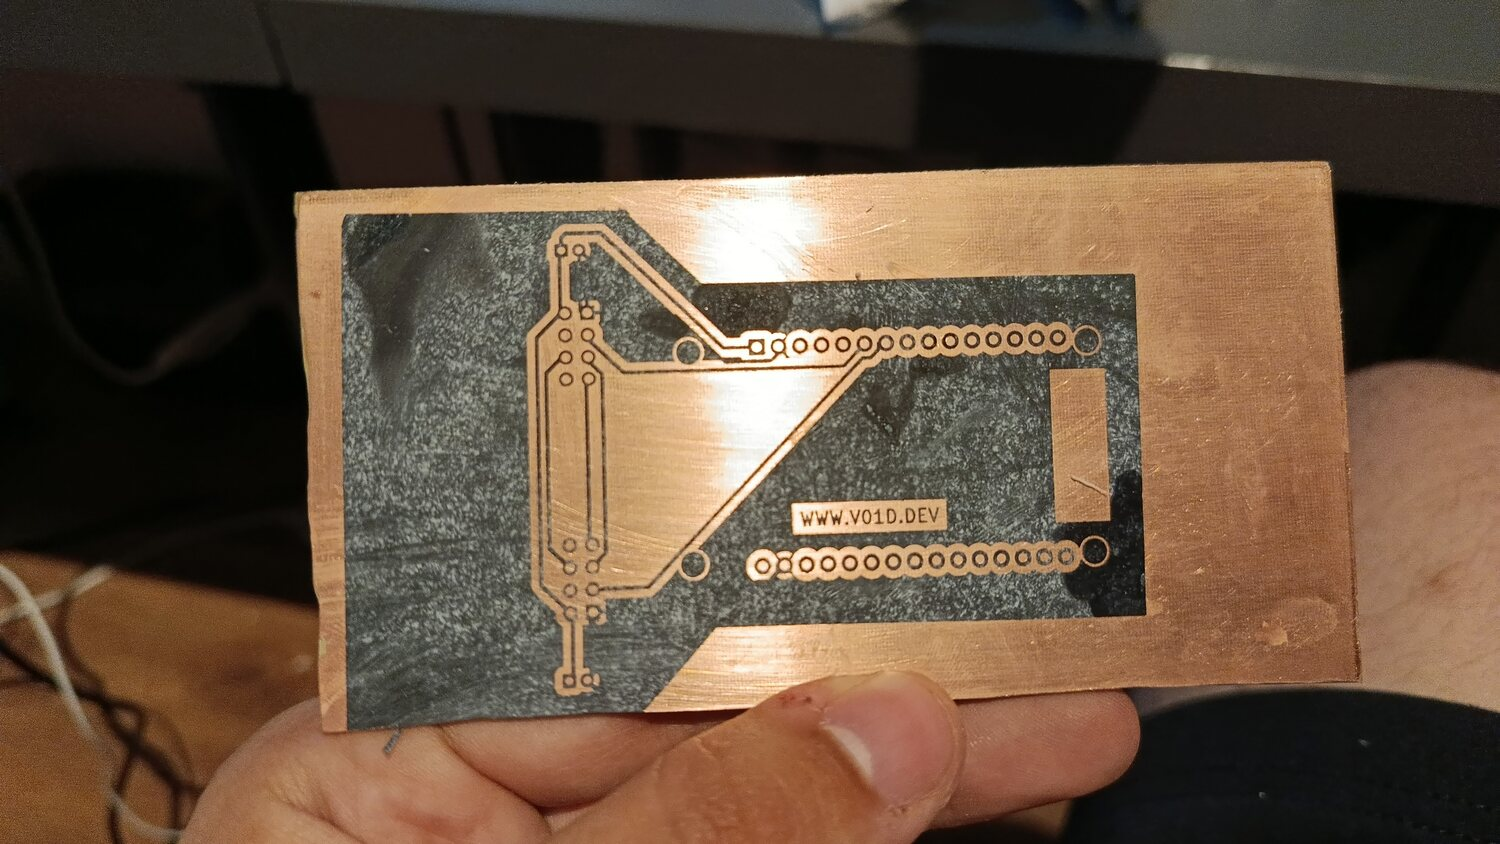
\includegraphics[width=0.35\textwidth]{../img/rf-transfer.jpg}
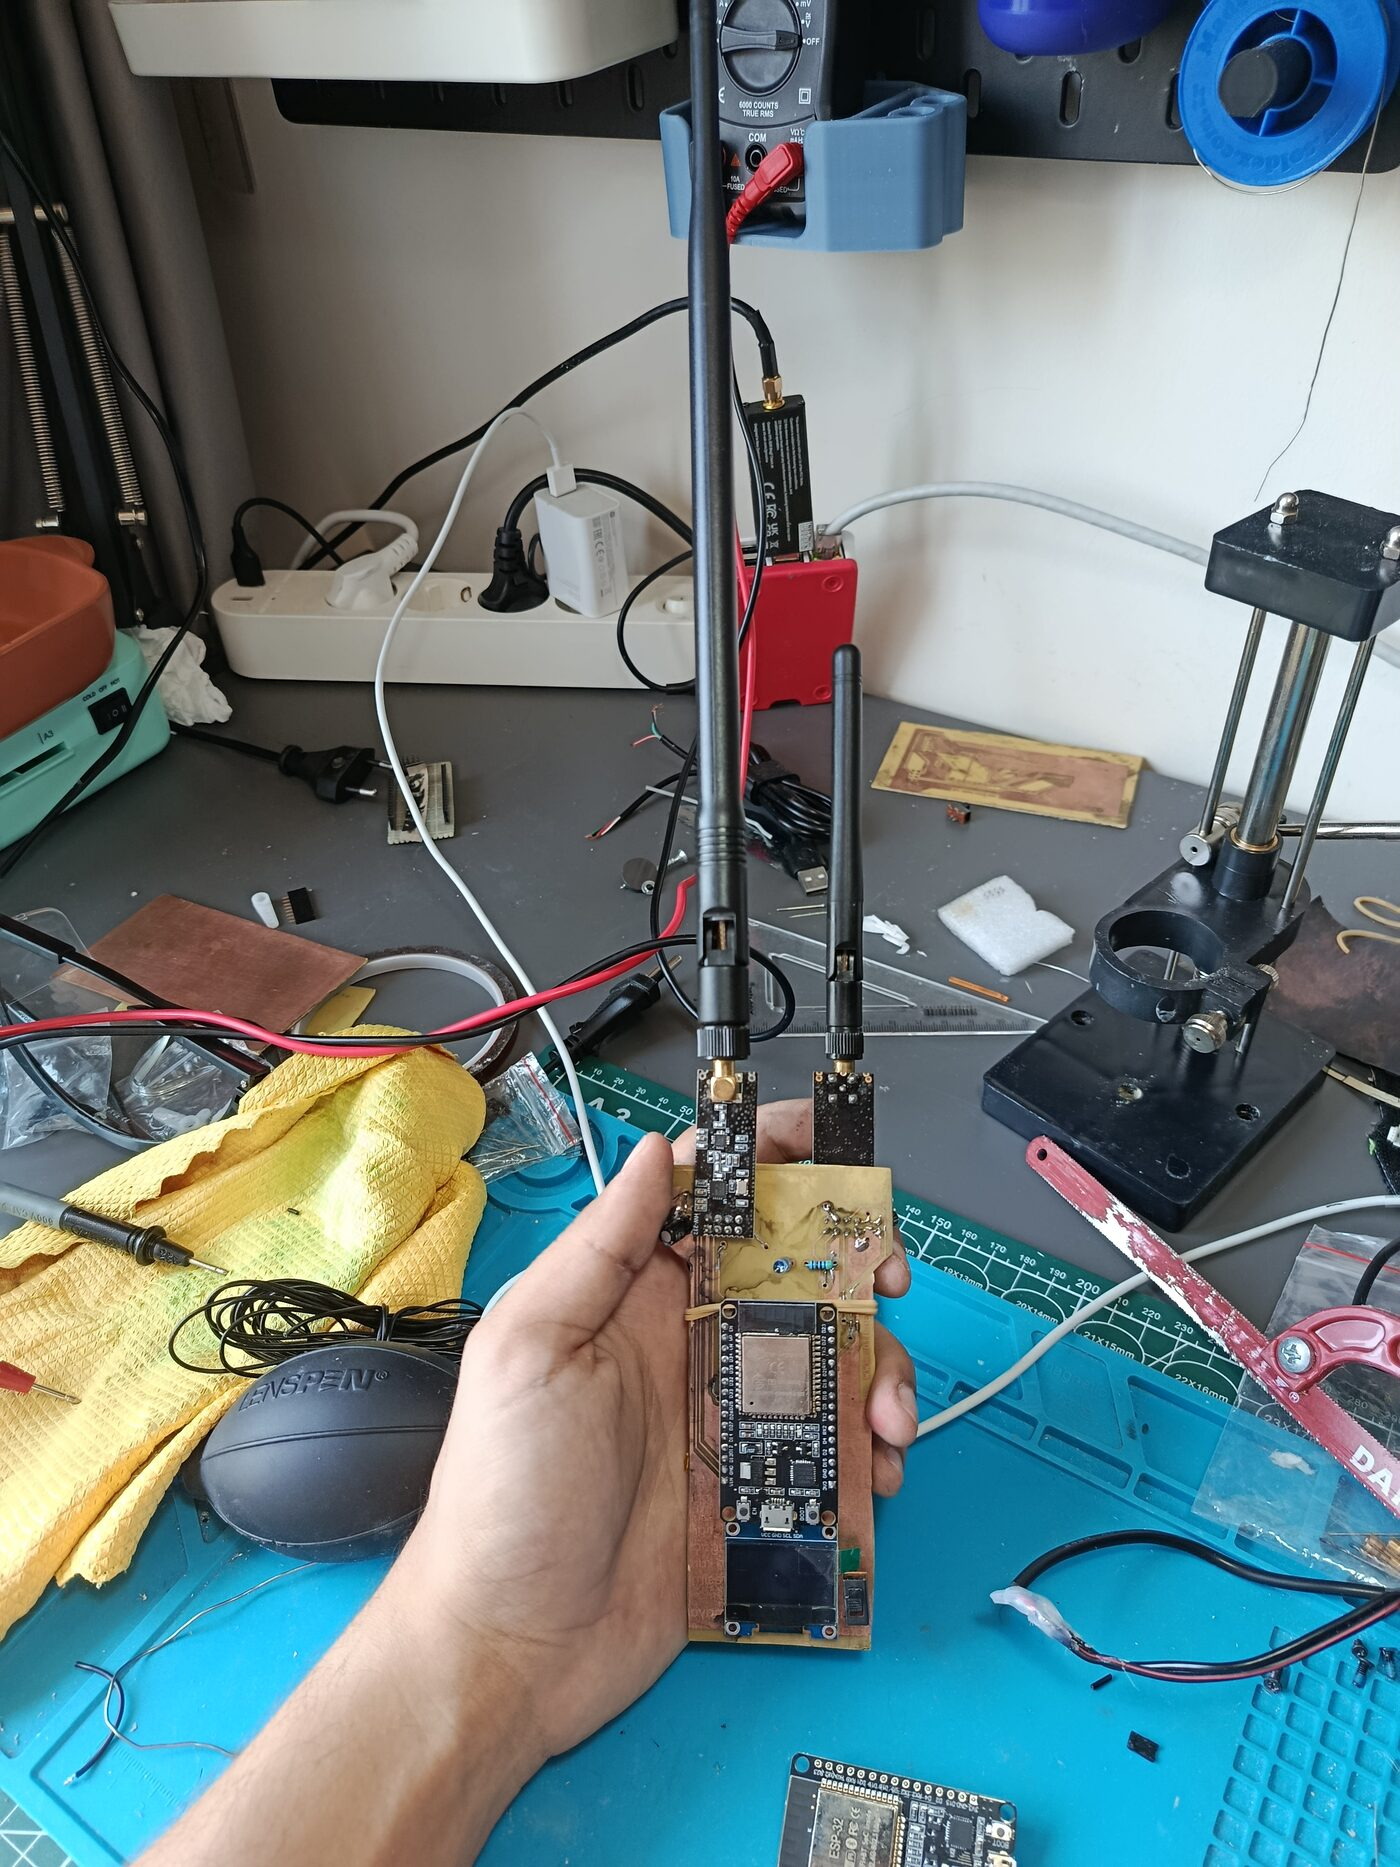
\includegraphics[width=0.25\textwidth]{../img/rf-board.jpg}\hspace{1.5em}%
\caption{The first revision: toner transferred onto copper, and the same board assembled.}
\end{figure}

\begin{figure}[!htbp]
\centering
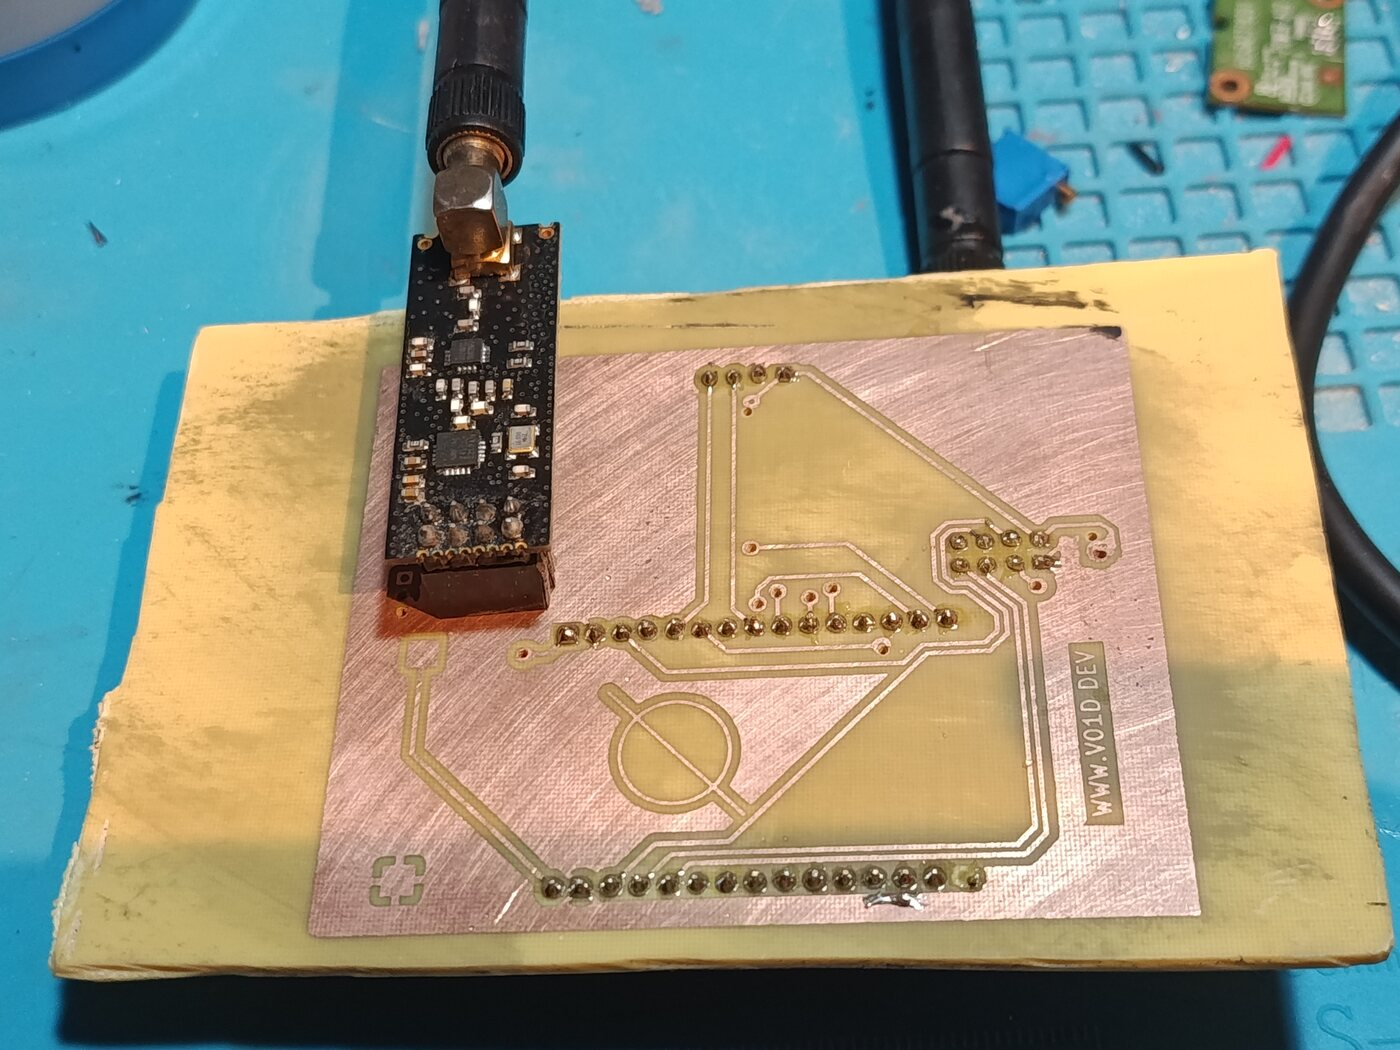
\includegraphics[width=0.31\textwidth]{../img/rf-etched.jpg}\hspace{1em}%
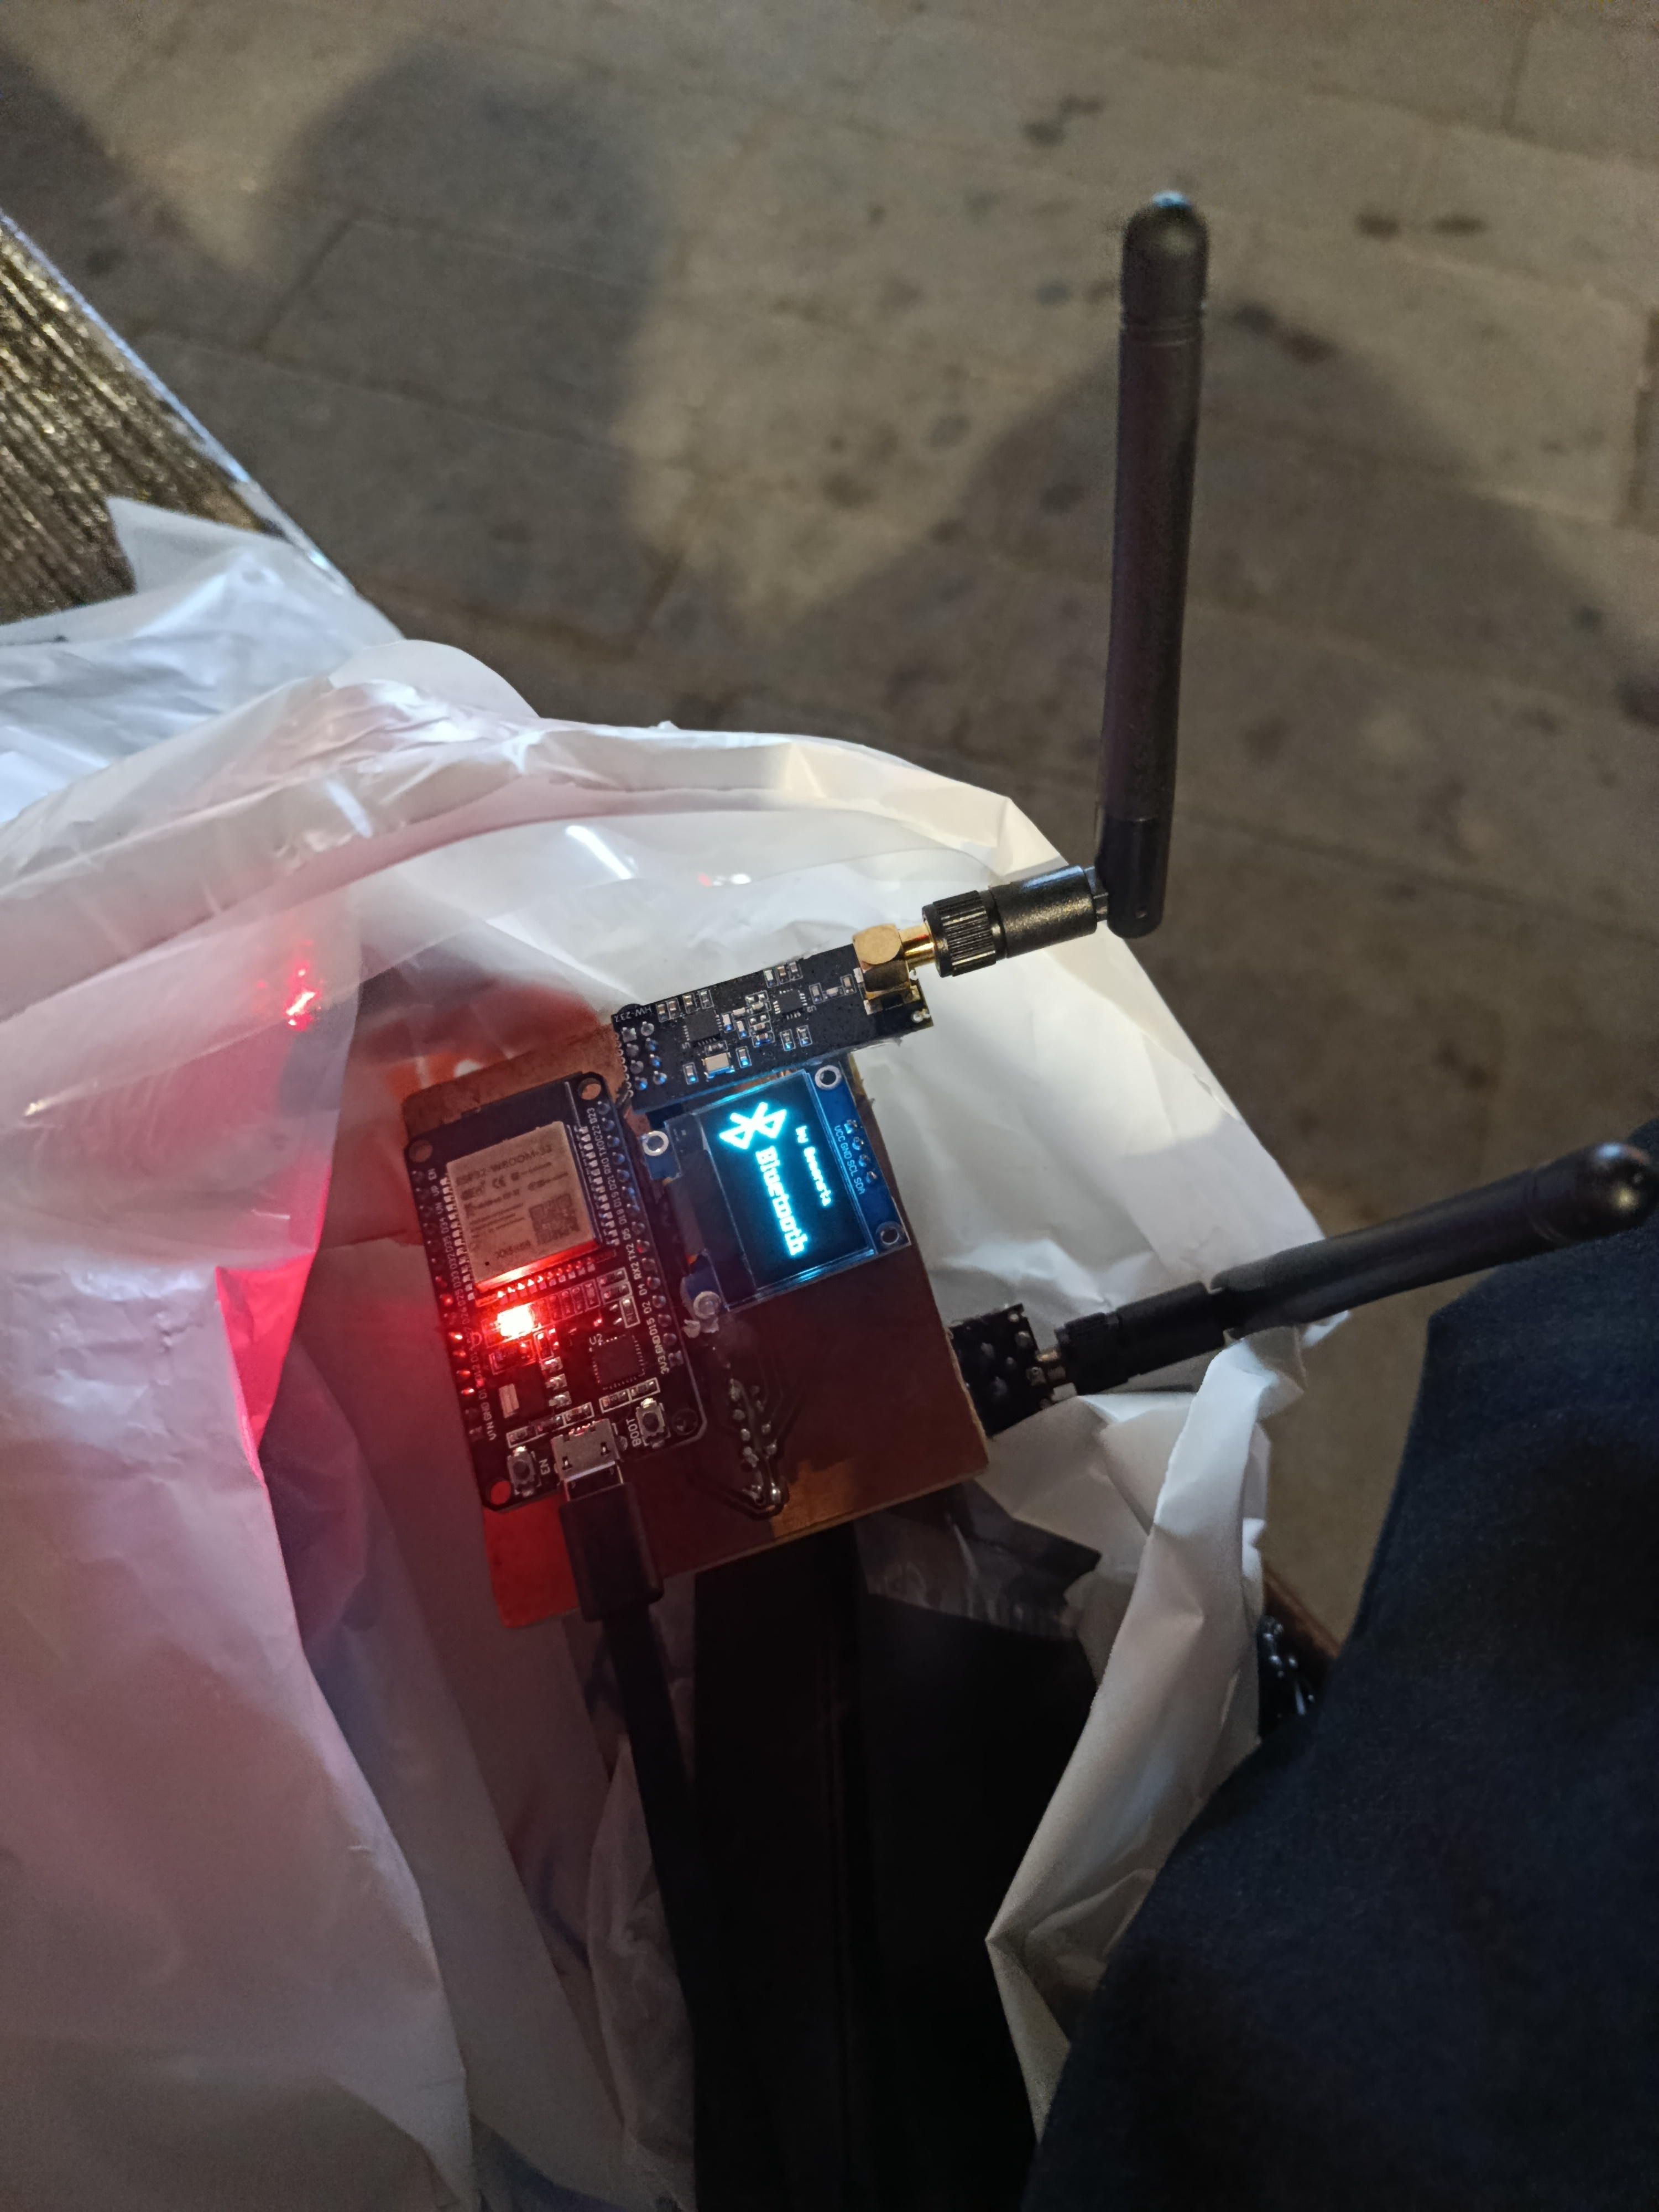
\includegraphics[width=0.31\textwidth]{../img/rf-final.jpg}
\caption{The final revision after etching, and the finished board in use.}
\end{figure}

\begin{figure}[!htbp]
\centering
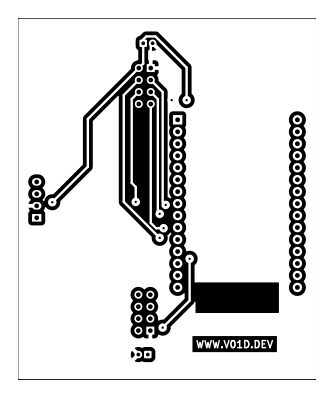
\includegraphics[width=0.17\textwidth]{../img/rf-fcu.png}\hspace{2.5em}%
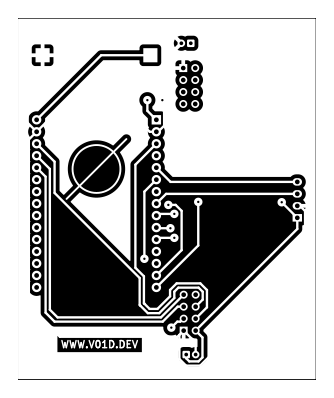
\includegraphics[width=0.17\textwidth]{../img/rf-bcu.png}
\caption{Front and back copper layers exported from KiCad. These are the etch artwork.}
\end{figure}

\entry{Flight Telemetry \& Attitude Indicator}{2026}

An ESP32 telemetry system for small aircraft, pairing an \textbf{MS5611}
barometer with an \textbf{MPU6050} inertial measurement unit. I fused the two
sensors through a complementary filter (to correct the gyroscope's drift against
the accelerometer's noise) and streamed attitude and altitude over serial at
roughly 50\,Hz.

The ground station is written in Python with \textbf{PySide6} and \textbf{Qt QML},
drawing a live artificial horizon from the incoming telemetry. I started it in
Pygame and migrated it to QML partway through, because the original approach
could not render smoothly enough to be useful as an instrument.

\begin{figure}[!htbp]
\centering
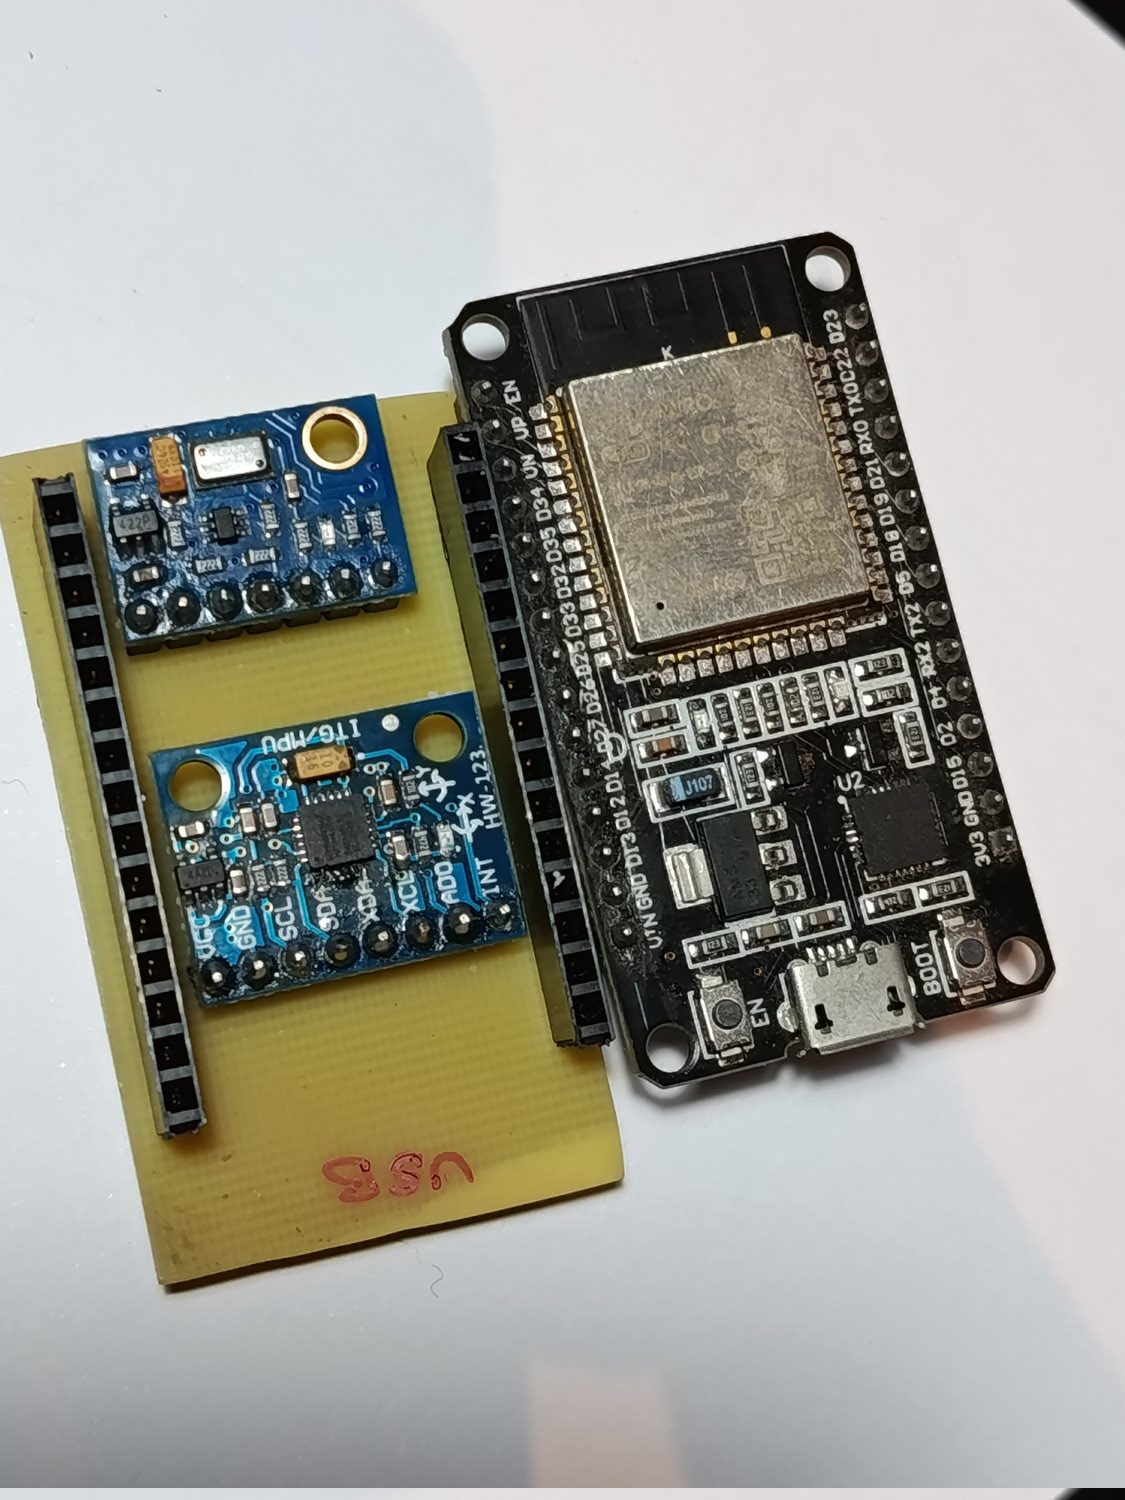
\includegraphics[width=0.30\textwidth]{../img/telemetry.jpg}
\caption{The telemetry board.}
\end{figure}

\entry{Discrete Transistor Logic Gates}{2026}

A board that implements \textbf{AND, NOT, OR and NAND} gates from individual
transistors, with no logic ICs anywhere: seven \textbf{PN2222A} NPN transistors
in resistor--transistor logic, with LEDs as outputs and tactile switches as
inputs.

I built this to work below the abstraction layer. It is easy to use a 74-series
chip and never think about what is inside it. Designing the same gates from
transistors means reasoning about base current, saturation and voltage levels
directly. I designed the schematic, routed the two-layer board with a ground
plane, and fabricated the first revision. It is currently under debug, and I am
working through the fault.

\begin{figure}[!htbp]
\centering
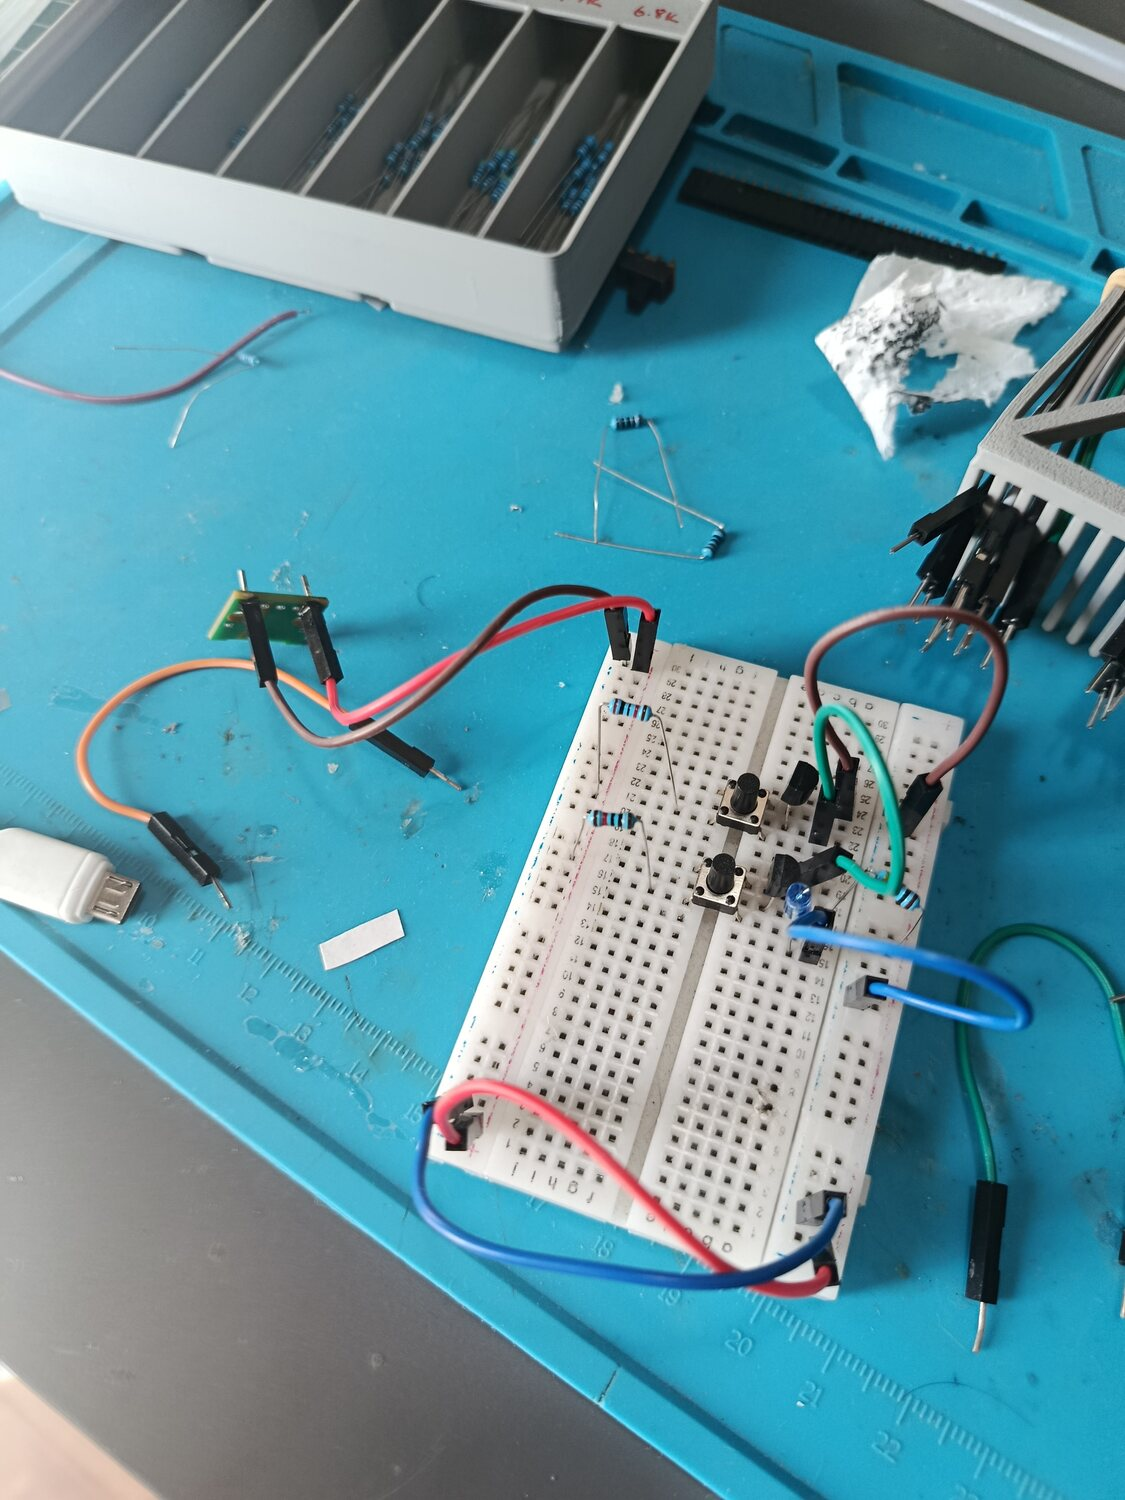
\includegraphics[width=0.38\textwidth]{../img/logic-gates.jpg}
\caption{The gate circuits on a breadboard, before committing to the PCB.}
\end{figure}

\entry{RC Aircraft \& Radio Link}{2025--2026}

Two fixed-wing designs, drawn and built from first principles rather than from a
kit. \textbf{FCF-1} uses a 9\,mm carbon fibre main spar with a \textbf{NACA 63412}
airfoil, and I modelled the airframe in \textbf{FreeCAD}: wing structure, servo
mounts, pushrods, control horns, aileron hinges and motor mount, all as parts
that could actually be cut and printed. It has flown. A later design,
\textbf{Simple-Glider}, was built to be easy to reproduce from foam board and
printed parts, with a full build guide covering dimensions and part counts.

For the radio link on these aircraft I wrote the transmitter and receiver
firmware myself: four analog channels encoded over \textbf{ESP-NOW} at 20\,Hz,
driving servos on the receiving end, with a failsafe that recentres every channel
if the link is lost for three seconds.

\entry{Published KiCad Library}{2026}

The SSD1306 0.96-inch OLED module is one of the most common parts in hobby
electronics, and I could not find a KiCad symbol and footprint for it that
worked in a current version of KiCad. So I made one and published it: a native
\textbf{KiCad 9} symbol and footprint, converted from an earlier library with
the original \textbf{CC BY-NC-SA} attribution preserved as its licence requires.

It is not a file sitting in a drawer. I use this footprint in my own boards,
including the RF board above.

\entry{Home PCB Fabrication}{ongoing}

Everything with a circuit board in this portfolio was made by hand, and the
process itself has been a project. I generate artwork from KiCad, transfer it to
copper, etch, drill and assemble, and I designed for that process on the boards
above. I modelled a \textbf{toner transfer tool} in FreeCAD specifically for
this workflow, and I write up the method on my site because the information that
helped me most came from other people doing the same thing.

I also model and print mechanical parts, from enclosures for the boards above to
a reversible USB power modification for a FlySky i6X transmitter that fits into
the battery compartment without altering the case.

\entry{Router Firmware Reverse Engineering}{2026}

I took a Xiaomi router apart to understand how it boots. I located the UART
header on the board and connected to it to capture the boot log, which is the
most direct way to see what a device does before any of its own software takes
over. The console turned out to be locked, so I moved to the flash instead and
extracted the firmware image, which showed the firmware was built on an
open-source base. I stopped there when the university term started.

\begin{figure}[!htbp]
\centering
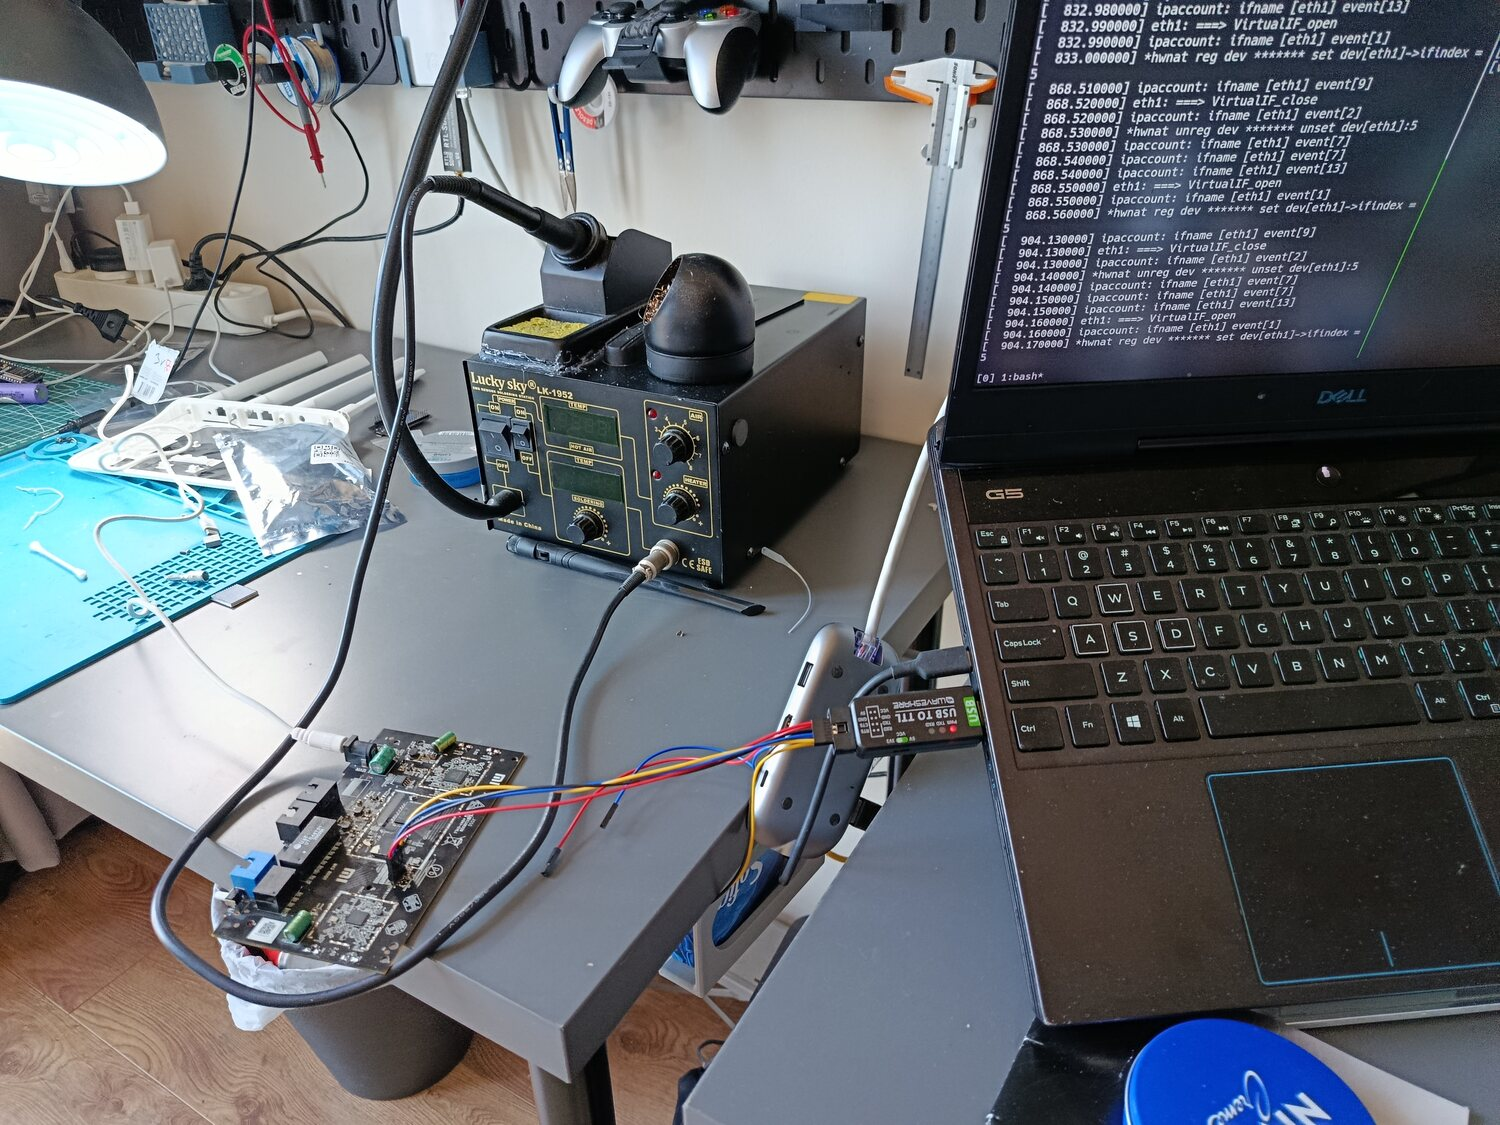
\includegraphics[width=0.40\textwidth]{../img/router-uart.jpg}
\caption{Capturing the boot log over UART.}
\end{figure}

\vspace{8pt}
\hrule
\vspace{6pt}

\textbf{Toolchain.} C and C++ on ESP32 and ESP8266, and Python for host-side
tooling. KiCad 9/10 for schematic capture and PCB layout, including custom
symbol and footprint authoring. FreeCAD for mechanical design, FDM printing for
parts. SPI, I\textsuperscript{2}C, UART, PWM and ADC at the hardware level;
nRF24L01, ESP-NOW, ExpressLRS, Bluetooth and IR for radio. Bench work with a
soldering iron, multimeter and serial telemetry.

\end{document}
